\documentclass[submit]{../harvardml}
% \documentclass[submit]
% \course{CS1810-S25}
\assignment{Homework \#4}
\duedate{April 3, 2026 at 11:59pm}

\usepackage[OT1]{fontenc}
\usepackage[colorlinks,citecolor=blue,urlcolor=blue]{hyperref}
\usepackage[pdftex]{graphicx}
\usepackage{caption}
\usepackage{fullpage}
\usepackage{soul}
\usepackage{amsmath}
\usepackage{amssymb}
\usepackage{framed}
\usepackage{color}
\usepackage{todonotes}
\usepackage{listings}
\usepackage{../common}
\usepackage{float,booktabs}
% Figures exported from the notebook (PDF/PNG) — place files under ./figures/
\graphicspath{{./figures/}}
\newcommand{\E}{\mathbb{E}}
\newcommand{\KL}{D_{\mathrm{KL}}}
\newcommand{\R}{\mathbb{R}}
\newcommand{\bx}{\mathbf{x}}
\newcommand{\bz}{\mathbf{z}}

%%%%%%%%%%%%%%%%%%%%%%%%%%%%%%%%%%%%%%%%%%%
%% Solution environment
\usepackage{xcolor}
\newenvironment{solution}{
    \vspace{2mm}
    \color{blue}\noindent\textbf{Solution}:
}{}
%%%%%%%%%%%%%%%%%%%%%%%%%%%%%%%%%%%%%%%%%%%

\usepackage[mmddyyyy,hhmmss]{datetime}

\definecolor{verbgray}{gray}{0.9}

\lstnewenvironment{csv}{
  \lstset{backgroundcolor=\color{verbgray},
  frame=single,
  framerule=0pt,
  basicstyle=\ttfamily,
  columns=fullflexible}}{}
 
\begin{document}

\begin{center}
{\Large Representation Learning, Transformers, and Non-parametric methods}\\
\end{center}

\subsection*{Introduction}

This homework contains three problems:
\begin{enumerate}
    \item You will do some transformer computations by hand, and implement self-attention from scratch and produce attention score heatmaps.
    \item You will do some derivations related to autoencoders and implement them.
    \item You will do some math to prove bounds on decision tree ensembles, in order to 
\end{enumerate}

We note that this homework does not have any problem where you directly run through the computations you would do to derive a decision tree. Doing so can be good review, however, so for an example with those computations, please see the last exercise in Section 6 notes.

\subsection*{Resources and Submission Instructions}

Please type your solutions after the corresponding problems using this \LaTeX\ template, and start each main problem on a new page.

Please submit the writeup PDF to the Gradescope assignment `HW4'. Remember to assign pages for each question.  \textbf{You must include any plots in your writeup PDF. }. Please submit your \LaTeX file and code files to the Gradescope assignment `HW4 - Supplemental.' The supplemental files will only be checked in special cases, e.g. honor code issues, etc. Your files should be named in the same way as we provide them in the repository, e.g. \texttt{hw4.pdf}, etc.




\newpage

%%%%%%%%%%%%%%%%%%%%%%%%%%%%%%%%%%%%%%%%%%%%%
% Problem : Understanding the Transformer
%%%%%%%%%%%%%%%%%%%%%%%%%%%%%%%%%%%%%%%%%%%%%

\begin{problem}[Understanding the Transformer, 40 pts]

Transformers are the dominant architecture behind large language models and many modern
sequence processing systems.  At the heart of every transformer is \textbf{self-attention},
a mechanism that allows each position in a sequence to ``look at'' every other position
and decide how much information to gather from each.

In this problem you will (a)~work through the math of scaled dot-product attention,
(b)~understand key design choices, and (c)~implement the attention layer.

\medskip\noindent
\textbf{Background.}
Given an input matrix $\boldX \in \reals^{T \times d}$ (one row per token),
self-attention computes:
\[
  \text{Attention}(\boldQ, \boldK, \boldV)
  = \text{softmax}\!\left(\frac{\boldQ \boldK^\trans}{\sqrt{d_k}}\right)\boldV,
\]
where $\boldQ = \boldX \boldW_Q$, $\boldK = \boldX \boldW_K$,
$\boldV = \boldX \boldW_V$ with learnable weight matrices
$\boldW_Q, \boldW_K \in \reals^{d \times d_k}$ and
$\boldW_V \in \reals^{d \times d_v}$.
The softmax is applied row-wise: for a row vector $\boldz \in \reals^T$,
$\text{softmax}(\boldz)_i = e^{z_i} / \sum_{j=1}^{T} e^{z_j}$.

\begin{enumerate}

%%% Part (a) %%%
\item \textbf{[10 pts] Attention by hand.}

Consider a sequence of $T = 2$ tokens with embedding dimension $d = 2$. The input
matrix, query weight matrix, key weight matrix, and value weight matrix are:
\[
  \boldX = \begin{pmatrix} 1 & 0 \\ 0 & 1 \end{pmatrix}, \quad
  \boldW_Q = \begin{pmatrix} 1 & 1 \\ 0 & 1 \end{pmatrix}, \quad
  \boldW_K = \begin{pmatrix} 1 & 0 \\ 1 & 1 \end{pmatrix}, \quad
  \boldW_V = \begin{pmatrix} 2 & 0 \\ 0 & 1 \end{pmatrix}.
\]
So $d_k = d_v = 2$.

\begin{enumerate}
  \item Compute $\boldQ$, $\boldK$, $\boldV$, and the raw score matrix
  $\boldS = \boldQ \boldK^\trans$.

  \item Compute the scaled score matrix $\boldS / \sqrt{d_k}$.
  Then apply softmax row-wise to obtain the attention weight matrix
  $\boldA \in \reals^{2 \times 2}$.

  You may leave your answer in terms of $e^{(\cdot)}$ and sums, or compute
  decimal approximations.
\end{enumerate}
%%% Part (b) %%%
\item \textbf{[5 pts] Why scale by $\sqrt{d_k}$\,?}

Suppose the entries of $\boldq, \boldk \in \reals^{d_k}$ are independent random
variables with mean~$0$ and variance~$1$.

\begin{enumerate}
  \item Compute the mean and variance of the dot product
  $\boldq^\trans \boldk = \sum_{i=1}^{d_k} q_i k_i$.

  \item As $d_k$ grows, what happens to the magnitude of $\boldq^\trans \boldk$?
  Explain in one or two sentences what effect this has on the softmax distribution
  (i.e.\ does it become more uniform or more peaked?).

  \item Show that after scaling by $1/\sqrt{d_k}$ the dot product has variance~$1$
  regardless of $d_k$.
\end{enumerate}

%%% Part (c) %%%
\item \textbf{[5 pts] Permutation equivariance.}

Let $\boldP_\sigma \in \reals^{T \times T}$ be the permutation matrix corresponding
to a permutation $\sigma$ of $\{1, \dots, T\}$ (i.e.\ $(\boldP_\sigma)_{ij} =
\mathbf{1}[j = \sigma(i)]$).

\begin{enumerate}
  \item Show that self-attention (without positional encoding) is
  \textbf{permutation equivariant}: if we permute the input rows by replacing
  $\boldX$ with $\boldP_\sigma \boldX$, the output is permuted in the same way.
  That is, show
  \[
    \text{Attention}(\boldP_\sigma \boldX) = \boldP_\sigma \, \text{Attention}(\boldX).
  \]
  \textit{Hint}: What happens to $\boldQ$, $\boldK$, $\boldV$, and the softmax
  when you left-multiply $\boldX$ by $\boldP_\sigma$?

  \item Explain in two or three sentences why permutation equivariance is a
  problem for tasks like language modeling, where word order matters.

  \item The standard fix is to add a \textbf{positional encoding}
  $\boldP\boldE \in \reals^{T \times d}$ to the input:
  $\boldX' = \boldX + \boldP\boldE$.
  Why does this break permutation equivariance?
\end{enumerate}

%%% Part (d) %%%
\item \textbf{[10 pts] Implementing self-attention from scratch (code).}

In the accompanying notebook, implement single-head scaled dot-product self-attention
using \textbf{only NumPy} (do not use pre-existing implementations such as PyTorch and sklearn).

Your function should take:
\begin{itemize}
  \item $\boldX \in \reals^{T \times d}$: input embeddings
  \item $\boldW_Q \in \reals^{d \times d_k}$, $\boldW_K \in \reals^{d \times d_k}$,
        $\boldW_V \in \reals^{d \times d_v}$: weight matrices
\end{itemize}
and return:
\begin{itemize}
  \item $\text{output} \in \reals^{T \times d_v}$: the attention output
  \item $\text{weights} \in \reals^{T \times T}$: the attention weight matrix $\boldA$
\end{itemize}

\textbf{Implementation tips}:
\begin{itemize}
  \item For numerical stability, before applying softmax to a row~$\boldz$, subtract
  $\max(\boldz)$: compute $\text{softmax}(\boldz - \max(\boldz))$. (As an aside, note that this does not change the softmax function.)
  % \item Test your implementation against the provided test cases.
\end{itemize}

%%% Part (e) %%%
\item \textbf{[10 pts] Multi-head attention}

In the notebook, extend your implementation to \textbf{multi-head attention}
and use it inside a small transformer classifier trained on a synthetic
sequence dataset.

Given $h$ heads, each head
  uses its own $\boldW_Q^{(i)}, \boldW_K^{(i)} \in \reals^{d \times d_k}$ and
  $\boldW_V^{(i)} \in \reals^{d \times d_v}$, where $d_k = d_v = d / h$.
  The outputs of all heads are concatenated and projected:
  \[
    \text{MultiHead}(\boldX) = [\text{head}_1 \,;\, \cdots \,;\, \text{head}_h]\,
    \boldW_O,
  \]
  where $\boldW_O \in \reals^{d \times d}$.

After training, attach one learned attention matrix as a heatmap and
briefly describe what it suggests the model is attending to.


\end{enumerate}

\end{problem}


\newpage


\begin{solution}

\paragraph{1(a)(i).}
Row wise multiplication gives
\[
  Q = X W_Q = \begin{pmatrix} 1 & 1 \\ 0 & 1 \end{pmatrix}, \quad
  K = X W_K = \begin{pmatrix} 1 & 0 \\ 1 & 1 \end{pmatrix}, \quad
  V = X W_V = \begin{pmatrix} 2 & 0 \\ 0 & 1 \end{pmatrix}
\]
The raw scores are $S_{ij} = q_i^\trans k_j$ (dot product of row $i$ of $Q$ with row $j$ of $K$):
\[
  S = Q K^\trans = \begin{pmatrix} 1 & 2 \\ 0 & 1 \end{pmatrix}
\]

\paragraph{1(a)(ii).}
With $d_k = 2$, the scaled matrix is $S/\sqrt{d_k}$:
\[
  \frac{1}{\sqrt{2}}\begin{pmatrix} 1 & 2 \\ 0 & 1 \end{pmatrix}
  = \begin{pmatrix} 1/\sqrt{2} & \sqrt{2} \\ 0 & 1/\sqrt{2} \end{pmatrix}
\]
For row $i$, subtract the row max, exponentiate, and normalize. For row~1 the max is $\sqrt{2}$ at column~2, so the shifted row is $[-1/\sqrt{2},\,0]$ and
\[
  A_{1j} = \frac{e^{z_j - \max}}{\sum_k e^{z_k - \max}}, \quad
  A_{11} = \frac{e^{-1/\sqrt{2}}}{1 + e^{-1/\sqrt{2}}}, \quad A_{12} = \frac{1}{1 + e^{-1/\sqrt{2}}}
\]
Row~2 has the same shifted values $[-1/\sqrt{2},\,0]$, hence the same attention weights as row~1. Numerically $A_{11} \approx 0.33$, $A_{12} \approx 0.67$. The attention output is $A V$ (each row of $A$ times $V$).

\paragraph{1(b)(i).}
By linearity, $\E[q^\trans k] = \sum_i \E[q_i]\E[k_i] = 0$. Because $q_i k_i$ are independent with mean~$0$,
\[
  \mathrm{Var}(q^\trans k) = \sum_{i=1}^{d_k} \mathrm{Var}(q_i k_i)
  = \sum_{i=1}^{d_k} \E[q_i^2]\E[k_i^2] = d_k
\]

\paragraph{1(b)(ii).}
The typical magnitude of $q^\trans k$ grows like $\sqrt{d_k}$ (standard deviation $\sqrt{d_k}$). Large dot products drive softmax inputs into large positive and negative values, so the distribution becomes more peaked (nearly one-hot).

\paragraph{1(b)(iii).}
Scaling gives $(q/\sqrt{d_k})^\trans k = (q^\trans k)/\sqrt{d_k}$, which has variance $\mathrm{Var}(q^\trans k)/d_k = 1$.

\paragraph{1(c)(i).}
Let $\widetilde{X} = P_\sigma X$. Then $\widetilde{Q} = P_\sigma Q$, $\widetilde{K} = P_\sigma K$, $\widetilde{V} = P_\sigma V$. The score matrix becomes $\widetilde{S} = \widetilde{Q}\widetilde{K}^\trans = P_\sigma S P_\sigma^\trans$, so row~$i$ of $\widetilde{S}$ is row~$\sigma(i)$ of $S$ with columns permuted the same way. Softmax is applied row-wise, so $\widetilde{A} = P_\sigma A P_\sigma^\trans$. Then $\widetilde{A}\widetilde{V} = P_\sigma A V$. Thus $\mathrm{Attention}(P_\sigma X) = P_\sigma\,\mathrm{Attention}(X)$.

\paragraph{1(c)(ii).}
Permutation equivariance means the layer cannot tell which position is first or second, shuffling words shuffles outputs the same way. Language meaning depends on order, so the model must distinguish positions.

\paragraph{1(c)(iii).}
The positional matrix $P\,E$ assigns different vectors to different positions. Permuting rows of $X$ without permuting the same rows of $P\,E$ changes which position gets which encoding, so the input to attention is no longer a pure row-permutation of the original; equivariance fails.

\paragraph{1(d).}
Implemented in \texttt{hw4\_release.ipynb}, with row wise max subtracted softmax.

\paragraph{1(e).}
Training curves and a learned attention map are shown below. The model reaches high test accuracy on the synthetic task. The heatmap for head~0 suggests the \texttt{[CLS]} query places substantial mass on the position containing \texttt{VAL0}/\texttt{VAL1}, which carries the label, rather than on distractor noise tokens.

\begin{figure}[H]
  \centering
  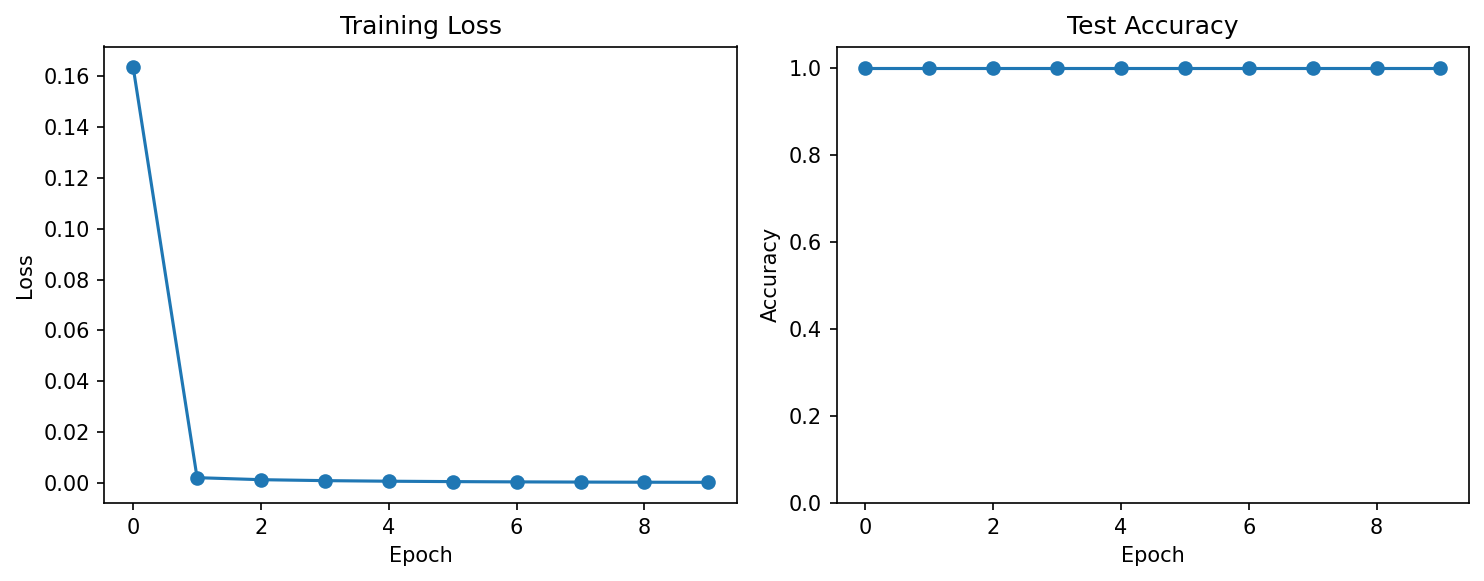
\includegraphics[width=0.9\linewidth]{p1_transformer_curves.png}
  \caption{Synthetic transformer: training loss and test accuracy.}
\end{figure}
\begin{figure}[H]
  \centering
  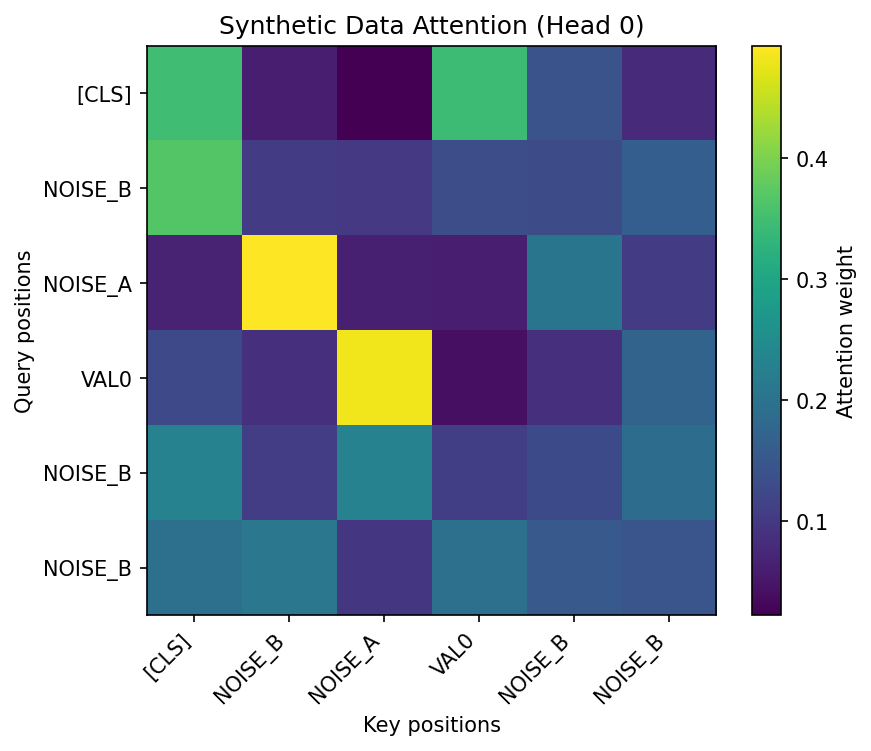
\includegraphics[width=0.75\linewidth]{p1_attention_head0.png}
  \caption{Attention weights (head 0) on one test sequence.}
\end{figure}

\end{solution}


\newpage



\begin{problem}[Autoencoders, 76 pts]
Suppose we want to compress our data into a lower-dimensional representation. What is a principled way to do this with machine learning, such that we can be confident the compression retains as much useful information as possible?

\begin{enumerate}
        \item The Autoencoder. 
        
We can turn this into a game between two networks. An \textit{encoder} $f_\phi : \mathbb R^n \to \mathbb R^d$ takes an input $\mathbf x$ and compresses it down to $d$ dimensions: $\mathbf z = f_\phi(\mathbf x)$. A \textit{decoder} $g_\theta : \mathbb R^d \to \mathbb R^n$ must then reconstruct the original input from just this compressed representation: $\hat{\mathbf x} = g_\theta(\mathbf z)$. We measure how well the decoder succeeds by comparing $\hat{\mathbf x}$ to $\mathbf x$, and backpropagate through both networks:
\[
  \mathcal{L}_{\mathrm{recon}} = \frac{1}{N}\sum_{i=1}^{N} \|\mathbf x_i - g_\theta(f_\phi(\mathbf x_i))\|^2.
\]
This is the \textit{reconstruction loss}, and it is the core of how autoencoders are trained. The logic is simple: if the decoder can faithfully recover $\mathbf x$ from $\mathbf z$, then $\mathbf z$ must have captured the essential structure of $\mathbf x$.

Note that what makes a model an ``autoencoder'' is this encoder--decoder coupling trained with a reconstruction loss---not any particular architecture. The encoder and decoder can be MLPs, CNNs, Transformers, or anything else. It is the training paradigm that defines the autoencoder.

\begin{enumerate}

\item \textbf{Implementation}[12 pts]. In the notebook, implement a convolutional autoencoder on CelebA. Train it, and provide your training and test loss curves. Display the first 5 test images alongside their reconstructions.

\item \textbf{Sampling}[4 pts]. In the notebook, sample random vectors $\mathbf z \sim \mathcal{N}(\bm{0}, \mathbf{I})$ from the autoencoder's latent space and decode them. Do the outputs look like faces? In 1--2 sentences, explain why the autoencoder has no reason to make its latent space produce coherent outputs when sampled this way.
\end{enumerate}
\item The autoencoder gives us a compressed representation, but its latent space has no structure that would let us \textit{generate} new data. What if, instead of learning point embeddings, we tried to learn the probability distribution over images, and then sample from it?

The natural objective is maximum likelihood: given a generative model with latent variables $\bz$ and a prior $p(\bz) = \mathcal{N}(\bm{0}, \mathbf{I})$, the log-likelihood of a datapoint $\bx$ is
\[
  \log p(\bx) = \log \int p(\bx, \bz)\, d\bz = \log \int p(\bx \mid \bz)\, p(\bz)\, d\bz.
\]

To train this model via maximum likelihood, we would need the true posterior $p(\bz \mid \bx)$. By Bayes' theorem,
\[
  p(\bz \mid \bx) = \frac{p(\bx \mid \bz)\, p(\bz)}{p(\bx)}.
\]
However, computing $p(\bx)$ (the evidence) requires evaluating the integral above over all possible values of $\bz$, which is intractable when $p(\bx \mid \bz)$ is parameterized by a neural network in high dimensions.

\begin{enumerate}

\item \textbf{Intractability}[4 pts]. In 1--2 sentences, explain concretely why the integral $\int p(\bx \mid \bz)\,p(\bz)\,d\bz$ is intractable. Why can't we just estimate it by drawing samples $\bz^{(k)} \sim p(\bz)$ and averaging $p(\bx \mid \bz^{(k)})$?
\end{enumerate}

Since we cannot compute $p(\bz \mid \bx)$ exactly, we introduce a neural network $q_\phi(\bz \mid \bx)$ that serves as an \textit{approximate posterior}---our best learned guess at the true posterior. To measure how well $q_\phi(\bz \mid \bx)$ approximates $p(\bz \mid \bx)$, we use the Kullback--Leibler (KL) divergence and once again need a clever technique:
\[
  \KL\!\big(q_\phi(\bz \mid \bx) \,\|\, p(\bz \mid \bx)\big) = \E_{q_\phi(\bz \mid \bx)}\!\Big[\log q_\phi(\bz \mid \bx) - \log p(\bz \mid \bx)\Big].
\]

\begin{enumerate}
\setcounter{enumii}{1}
\item \textbf{Deriving the ELBO.} Starting from the KL divergence above:

\begin{enumerate}
  \item \textbf{Expanding} [8 pts]. Expand $\log p(\bz \mid \bx)$ using Bayes' rule, and rearrange to show:
  \[
    \log p(\bx) = \KL\!\big(q_\phi(\bz \mid \bx) \,\|\, p(\bz \mid \bx)\big) + \E_{q_\phi(\bz \mid \bx)}\!\Big[\log p(\bx, \bz) - \log q_\phi(\bz \mid \bx)\Big].
  \]

  \item \textbf{Interpretation} [4 pts]. We define the second term to be the \textbf{Evidence Lower Bound (ELBO)}:
  \[
    \mathrm{ELBO} = \E_{q_\phi(\bz \mid \bx)}\!\Big[\log p(\bx, \bz) - \log q_\phi(\bz \mid \bx)\Big].
  \]
  Since $\KL \geq 0$, conclude that $\mathrm{ELBO} \leq \log p(\bx)$. In one sentence, explain why this means maximizing the ELBO is a sensible surrogate for maximizing the intractable log-likelihood.

  \item\textbf{Rewriting} [8 pts]. Now show that the ELBO can be rewritten as:
  \[
    \mathrm{ELBO} = \E_{q_\phi(\bz \mid \bx)}\!\big[\log p(\bx \mid \bz)\big] - \KL\!\big(q_\phi(\bz \mid \bx) \,\|\, p(\bz)\big).
  \]
  (Hint: split $\log p(\bx, \bz) = \log p(\bx \mid \bz) + \log p(\bz)$.)

\end{enumerate}

\item \textbf{Interpreting the VAE loss.} The loss we minimize is the negative ELBO:
\[
  \mathcal{L}_{\mathrm{VAE}} = -\E_{q_\phi(\bz \mid \bx)}\!\big[\log p(\bx \mid \bz)\big] + \KL\!\big(q_\phi(\bz \mid \bx) \,\|\, p(\bz)\big).
\]

\begin{enumerate}
  \item \textbf{Interpretation}[4 pts]. The first term is the (negative) expected log-likelihood of $\bx$ given samples from the encoder. In 1--2 sentences, explain how this connects back to the reconstruction loss from Section 1. What does minimizing it encourage?

  \item \textbf{Interpretation}[4 pts]. The second term penalizes the encoder's output distribution $q_\phi(\bz \mid \bx)$ for deviating from the prior $p(\bz) = \mathcal{N}(\bm{0}, \mathbf{I})$. Explain how this term addresses the problem you identified in question 1(b): why does it give the model an incentive to organize the latent space for generation?

  \item \textbf{Tensity}[4 pts]. These two terms pull in opposite directions. In 1--2 sentences, describe the qualitative effect of this tension on the VAE's reconstructions and generated samples, compared to the standard autoencoder.
\end{enumerate}

\end{enumerate}
\item VAE Implementation
%% ============================================================

In a VAE, the encoder outputs the parameters of the approximate posterior\\ $q_\phi(\bz \mid \bx) = \mathcal{N}(\bm{\mu}_\phi(\bx),\, \mathrm{diag}(\bm{\sigma}_\phi^2(\bx)))$. That is, a shared convolutional backbone produces a feature vector, which is then projected through two separate linear heads: one outputting $\bm{\mu} \in \R^d$ and one outputting $\log \bm{\sigma}^2 \in \R^d$. During training, we sample $\bz$ from this distribution; during generation, we sample $\bz \sim \mathcal{N}(\bm{0}, \mathbf{I})$ and decode.

\begin{enumerate}

\item \textbf{Reparameterization}[8 pts]. We need to backpropagate through the sampling step $\bz \sim q_\phi(\bz \mid \bx)$, but sampling is not differentiable.
 In 1--2 sentences, explain why we cannot directly backpropagate gradients through a sampling operation with respect to the distribution's parameters.
  Show that if $\bm{\epsilon} \sim \mathcal{N}(\bm{0}, \mathbf{I})$, then $\bz = \bm{\mu}_\phi(\bx) + \bm{\sigma}_\phi(\bx) \odot \bm{\epsilon}$ has distribution $q_\phi(\bz \mid \bx)$, and explain briefly why this makes the loss differentiable w.r.t.\ $\phi$.

\item \textbf{Closed-form KL}[6 pts]. Derive the closed-form expression for the KL term when $q = \mathcal{N}(\bm{\mu}, \mathrm{diag}(\bm{\sigma}^2))$ and $p = \mathcal{N}(\bm{0}, \mathbf{I})$:
\[
  \KL(q \| p) = \frac{1}{2}\sum_{j=1}^{d}\Big(\mu_j^2 + \sigma_j^2 - \ln \sigma_j^2 - 1\Big).
\]
(Hint: work coordinate-by-coordinate. Use $\E[z_j] = \mu_j$ and $\E[z_j^2] = \mu_j^2 + \sigma_j^2$.)

\item \textbf{Implementation}[12 pts]. In the notebook, implement a VAE using the architecture described above. Train it, and provide your training and test loss curves (decomposed into reconstruction and KL terms). Display the first 5 test images alongside their reconstructions. Then, sample from $\mathcal{N}(\bm{0}, \mathbf{I})$ and decode---do the samples look like faces? Compare to your results from 1(b).

\end{enumerate}
\end{enumerate}
\end{problem}

\newpage

\begin{solution}

\paragraph{1(a).}
Implemented in the notebook. convolutional encoder-decoder on CelebA with train/test MSE curves below, five test originals vs.\ reconstructions.

\begin{figure}[H]
  \centering
  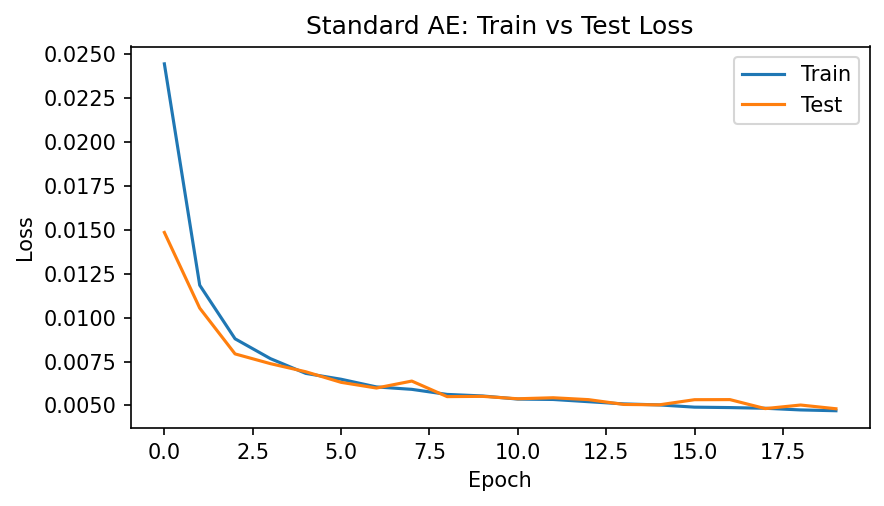
\includegraphics[width=0.85\linewidth]{ae_train_test_loss.png}
  \caption{Standard autoencoder: train vs.\ test reconstruction MSE.}
\end{figure}
\begin{figure}[H]
  \centering
  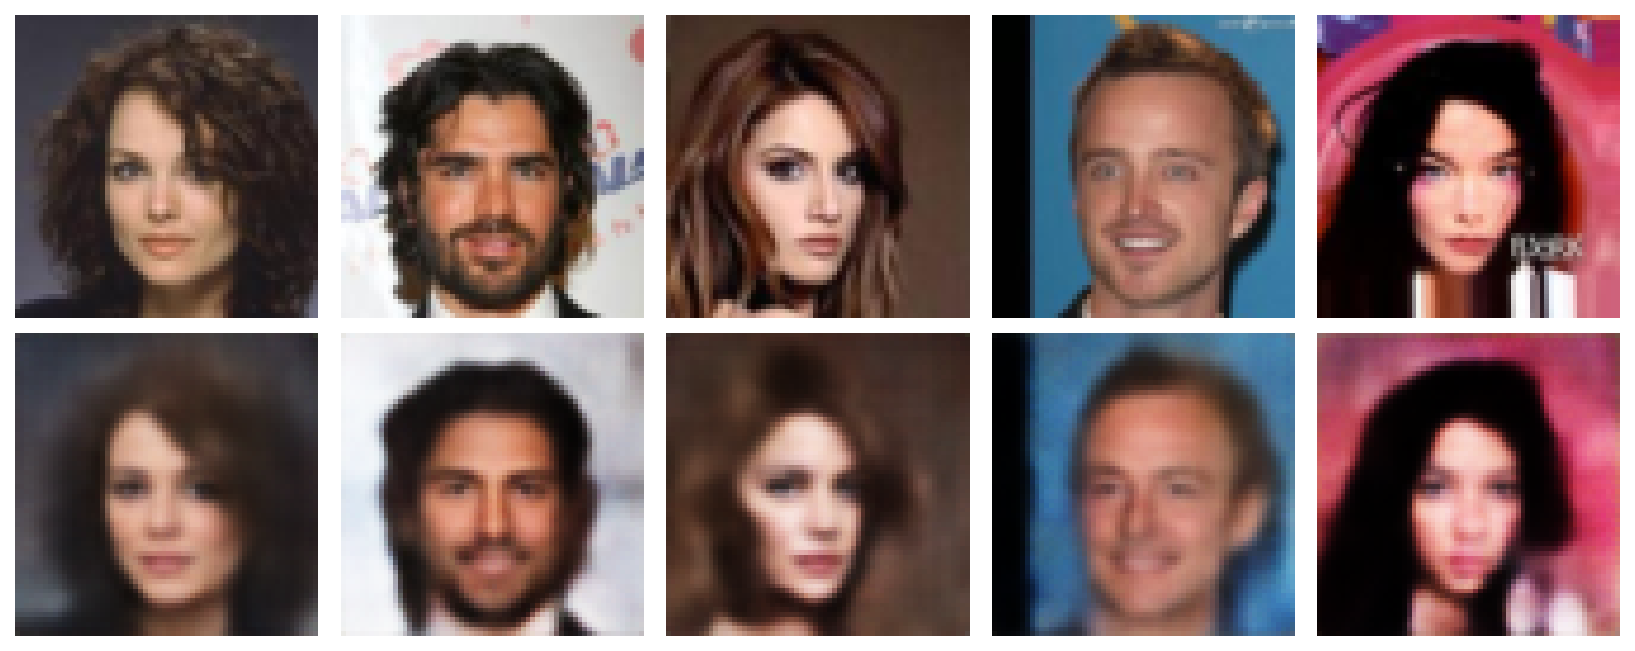
\includegraphics[width=0.95\linewidth]{ae_reconstructions.png}
  \caption{Five CelebA test images (top) and reconstructions (bottom).}
\end{figure}

\paragraph{1(b).}
Random $z \sim \mathcal{N}(0, I)$ decoded from the AE usually do not look like realistic faces (see figure). The AE is only trained to map each training image to some code and back, nothing forces those codes to cover $\R^d$ or to match the Gaussian prior, so most Gaussian draws lie in regions the decoder never learned to use.

\begin{figure}[H]
  \centering
  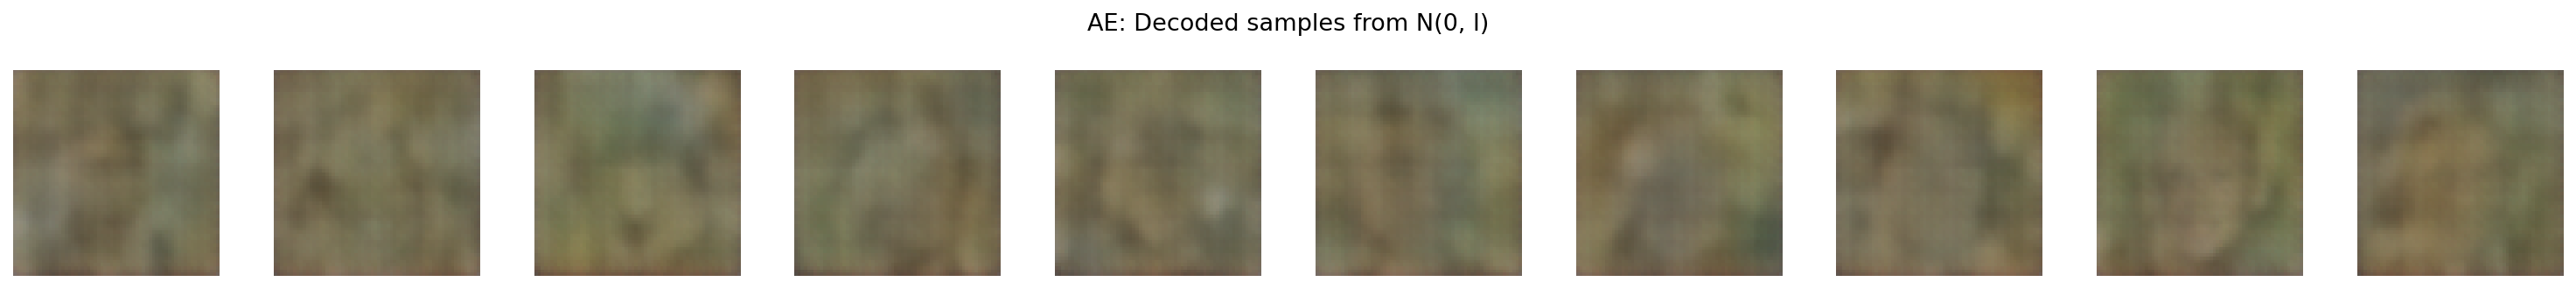
\includegraphics[width=0.95\linewidth]{ae_random_samples.png}
  \caption{AE: samples from $\mathcal{N}(0, I)$ passed through the decoder.}
\end{figure}

\paragraph{2(a).}
The integral $\int p(x \mid z)\,p(z)\,dz$ is a high-dimensional integral of a highly peaked neural likelihood against the prior; we cannot enumerate a grid. Monte Carlo with $z^{(k)} \sim p(z)$ estimates the average of $p(x \mid z)$, not the integral: the quantity $\E_{p(z)}[p(x \mid z)]$ differs from $p(x)$ by Jensen's gap for $\log$, and the variance of importance style estimators explodes when the prior samples rarely hit regions where $p(x \mid z)$ is large.

\paragraph{2(b)(i).}
Using Bayes rule, $\log p(z \mid x) = \log p(x \mid z) + \log p(z) - \log p(x)$. Substitute into the KL definition and expand the expectation:
\[
  \KL\!\big(q_\phi \,\|\, p(\cdot \mid x)\big)
  = \E_q\big[\log q_\phi(z \mid x) - \log p(x \mid z) - \log p(z)\big] + \log p(x)
\]
Rearranging yields
\[
  \log p(x) = \KL\!\big(q_\phi \,\|\, p(\cdot \mid x)\big) + \E_q\big[\log p(x, z) - \log q_\phi(z \mid x)\big]
\]

\paragraph{2(b)(ii).}
Since $\KL \geq 0$, the second term (ELBO) satisfies $\mathrm{ELBO} \leq \log p(x)$. Maximizing a lower bound on $\log p(x)$ pushes up the true likelihood whenever the bound is reasonably tight.

\paragraph{2(b)(iii).}
Split $\log p(x, z) = \log p(x \mid z) + \log p(z)$:
\[
  \mathrm{ELBO} = \E_q[\log p(x \mid z)] + \E_q[\log p(z) - \log q_\phi(z \mid x)]
  = \E_q[\log p(x \mid z)] - \KL\!\big(q_\phi \,\|\, p(z)\big)
\]

\paragraph{2(c)(i).}
With Gaussian decoder, $\log p(x \mid z)$ is (up to constants) negative squared error, minimizing $-\E_q[\log p(x \mid z)]$ is the same spirit as minimizing reconstruction MSE, encouraging accurate reconstructions from latent draws.

\paragraph{2(c)(ii).}
Matching $q_\phi$ to $\mathcal{N}(0, I)$ spreads mass so that sampling $z \sim \mathcal{N}(0, I)$ at test time lands in regions the decoder was trained to invert, addressing the unstructured latent of 1(b).

\paragraph{2(c)(iii).}
Strong reconstruction pushes informative but possibly irregular codes; the KL pulls codes toward the prior and can blur reconstructions while making samples more coherent than the plain AE.

\paragraph{3(a).}
A discrete draw $z \sim q_\phi$ does not depend smoothly on $(\mu, \sigma)$ in a way PyTorch can differentiate through. For $\epsilon \sim \mathcal{N}(0, I)$, the vector $z = \mu + \sigma \odot \epsilon$ is Gaussian with mean $\mu$ and diagonal variance $\sigma^2$; gradients flow through $\mu$ and $\sigma$ while $\epsilon$ is a fixed noise draw per forward pass.

\paragraph{3(b).}
Coordinatewise, $\KL(q_j \,\|\, p_j) = \tfrac{1}{2}\big(\mu_j^2 + \sigma_j^2 - \log \sigma_j^2 - 1\big)$, summing gives the stated formula.

\paragraph{3(c).}
VAE training curves (reconstruction, KL, total) and visual results are below. Random prior samples are more face like than the AE's because the KL term aligns the aggregate posterior with $\mathcal{N}(0, I)$.

\begin{figure}[H]
  \centering
  \begin{minipage}{0.32\linewidth}\centering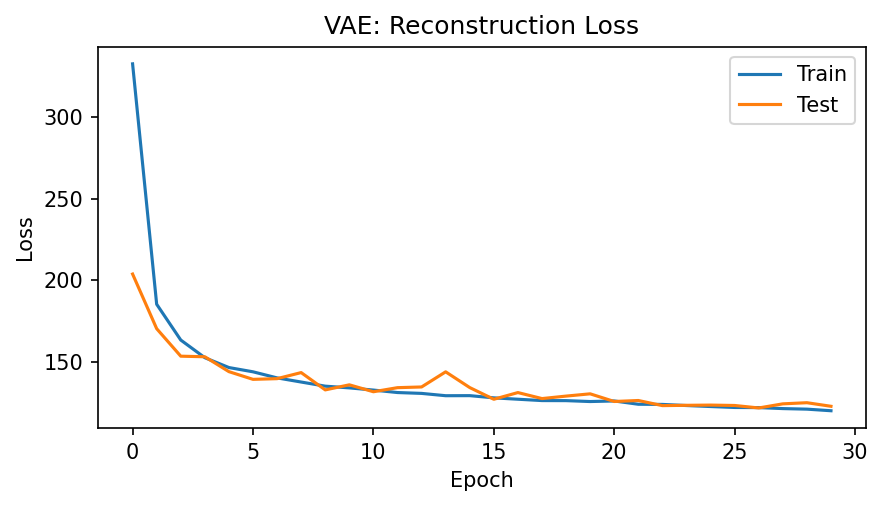
\includegraphics[width=\linewidth]{vae_recon_loss.png}\end{minipage}\hfill
  \begin{minipage}{0.32\linewidth}\centering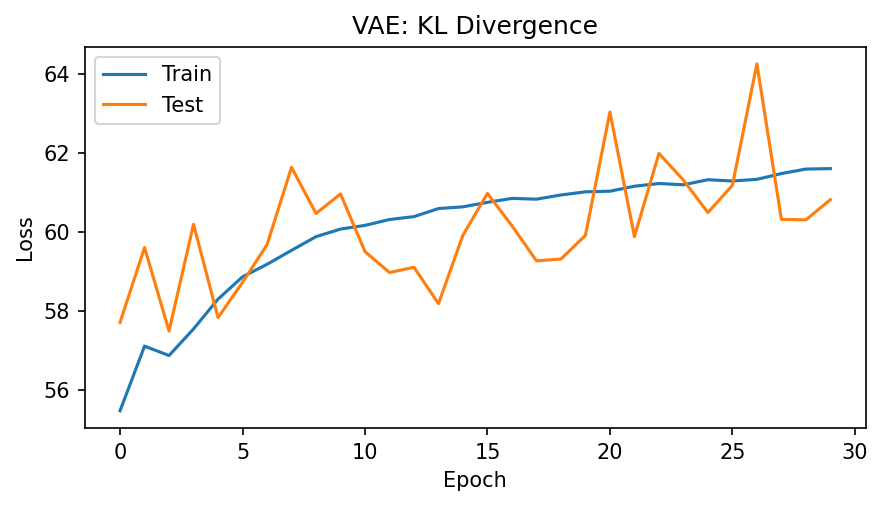
\includegraphics[width=\linewidth]{vae_kl.png}\end{minipage}\hfill
  \begin{minipage}{0.32\linewidth}\centering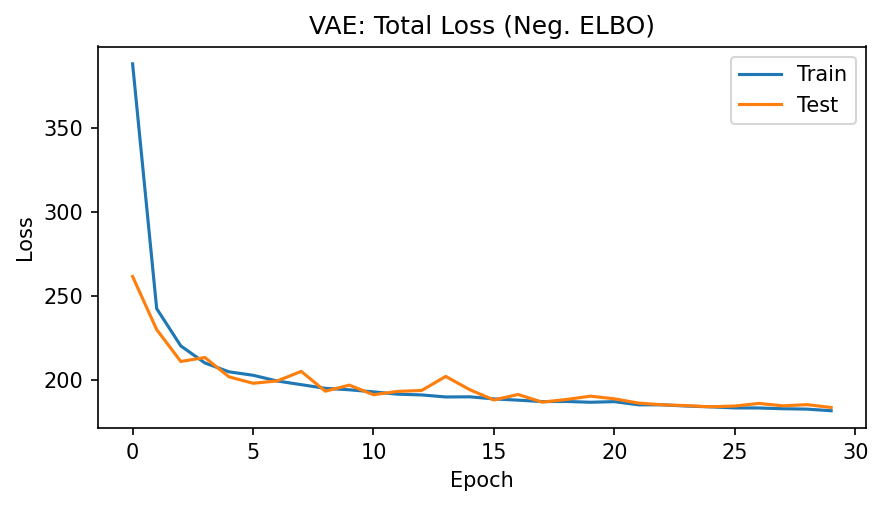
\includegraphics[width=\linewidth]{vae_total_loss.png}\end{minipage}
  \caption{VAE: reconstruction term, KL term, and total negative ELBO (train vs.\ test).}
\end{figure}
\begin{figure}[H]
  \centering
  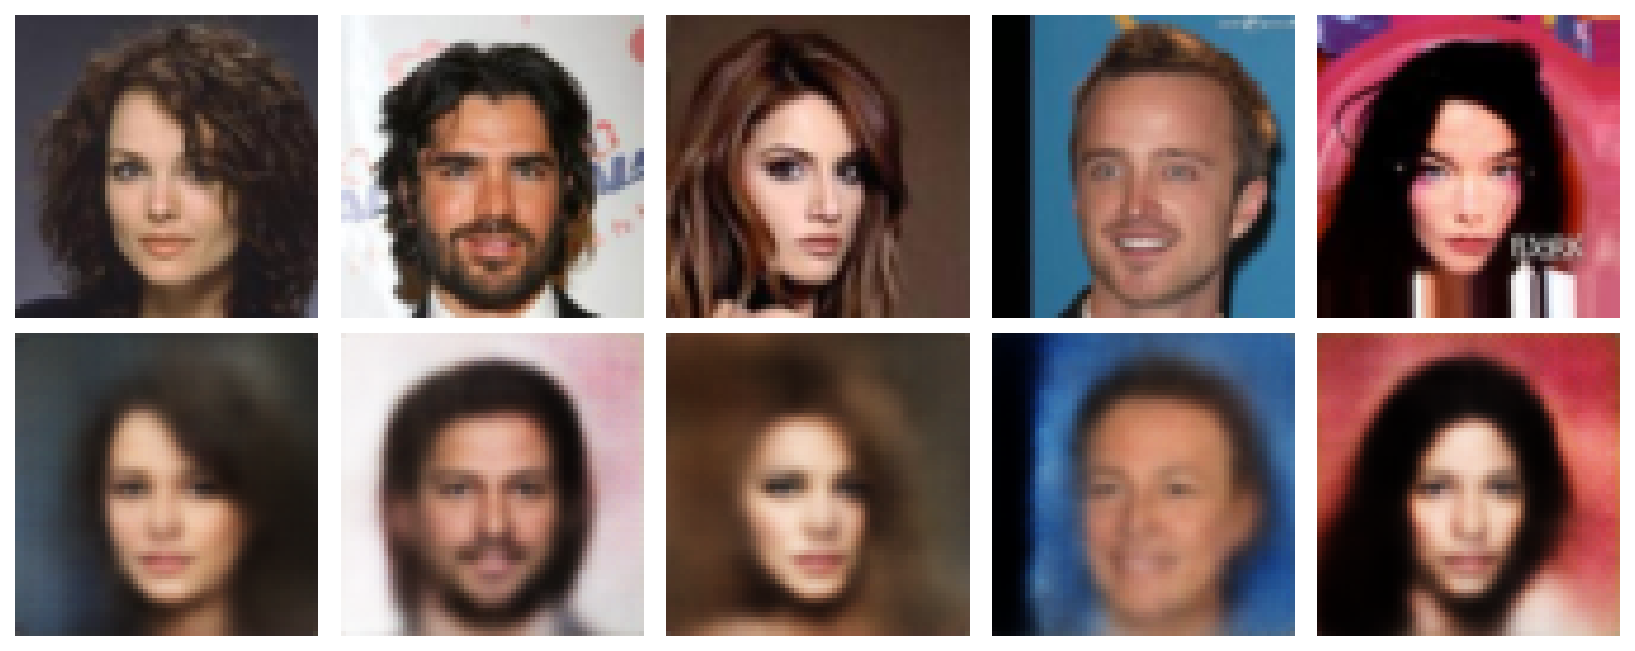
\includegraphics[width=0.95\linewidth]{vae_reconstructions.png}
  \caption{VAE: five test originals (top) and reconstructions (bottom).}
\end{figure}
\begin{figure}[H]
  \centering
  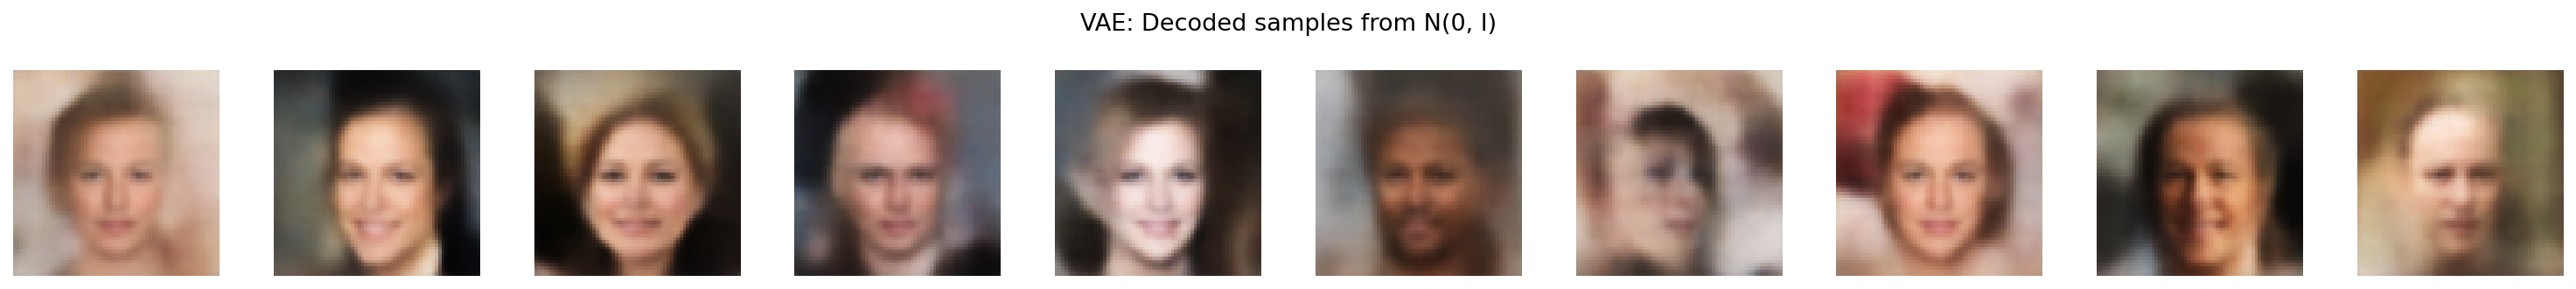
\includegraphics[width=0.95\linewidth]{vae_random_samples.png}
  \caption{VAE: decoding random $z \sim \mathcal{N}(0, I)$.}
\end{figure}

\paragraph{Part 4 (latent arithmetic).}
The notebook computes attribute direction vectors in latent space and applies \texttt{apply\_attribute} / \texttt{interpolate\_attribute}. Below are VAE and AE grids (negative / original / positive along each direction), then VAE interpolations along each direction.

\begin{figure}[H]
  \centering
  \begin{minipage}{0.48\linewidth}\centering
    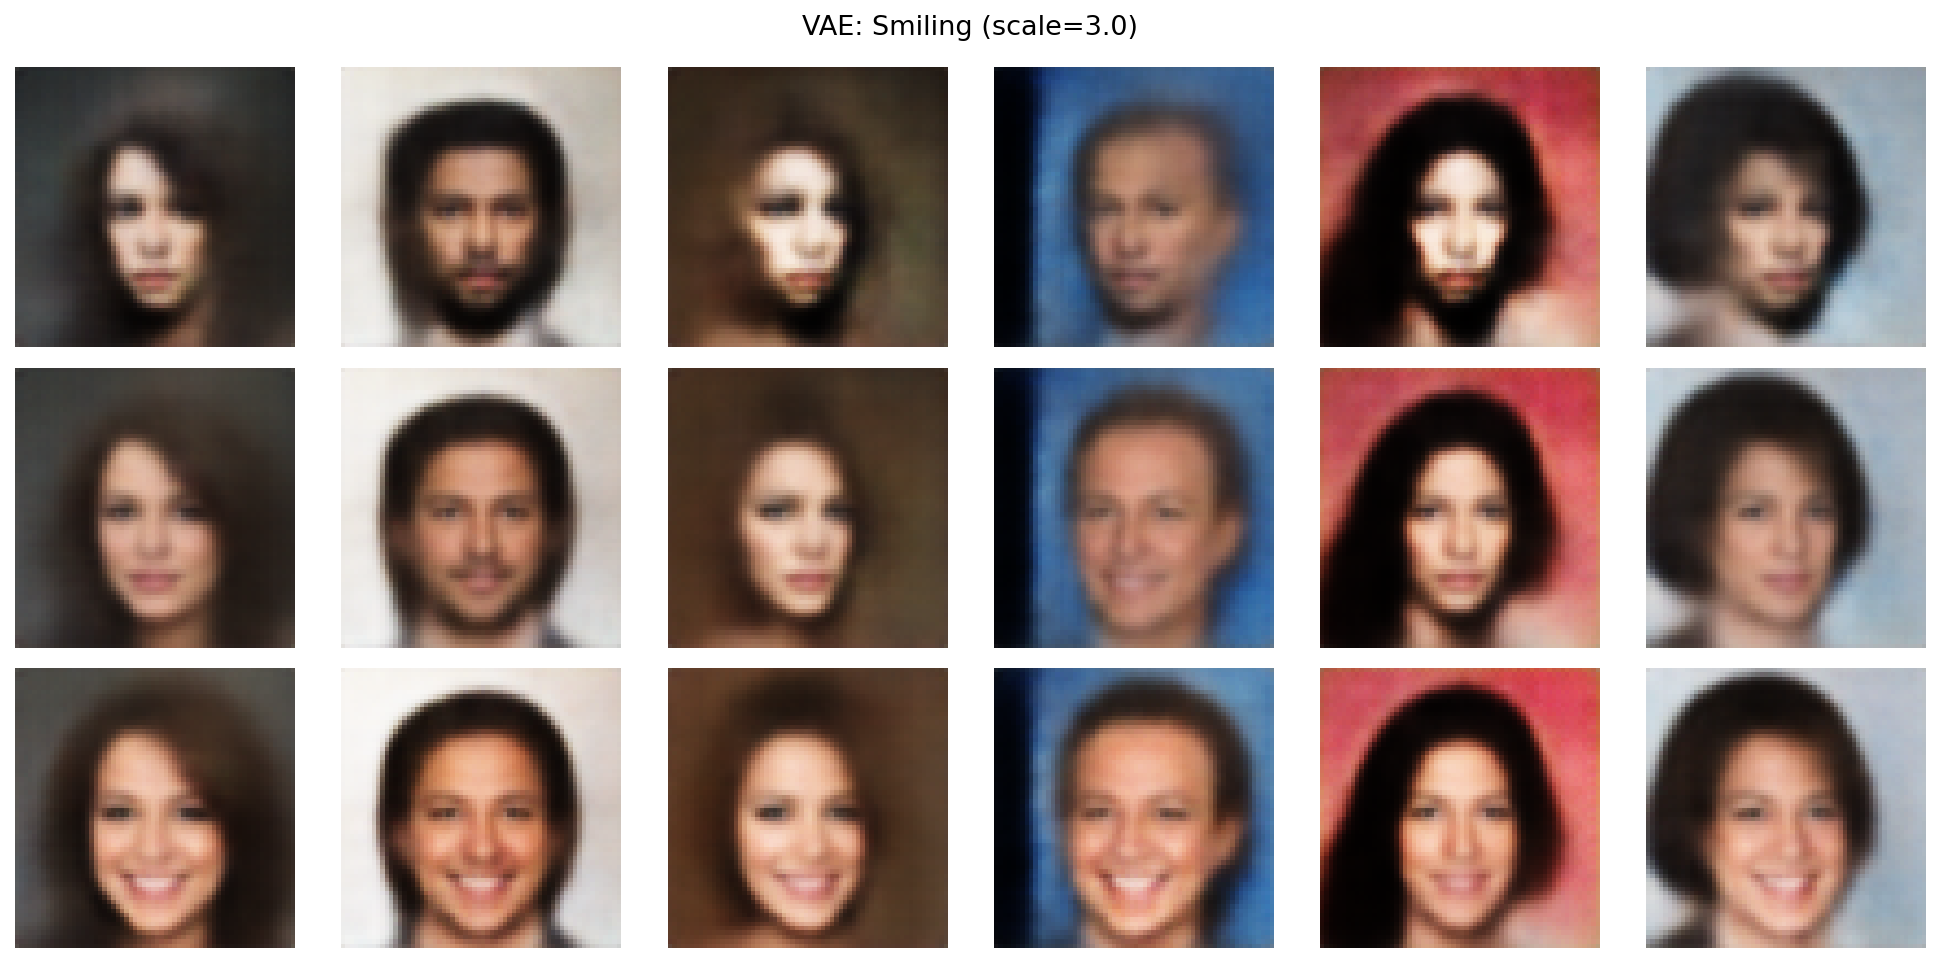
\includegraphics[width=\linewidth]{vae_attr_smiling.png}
  \end{minipage}\hfill
  \begin{minipage}{0.48\linewidth}\centering
    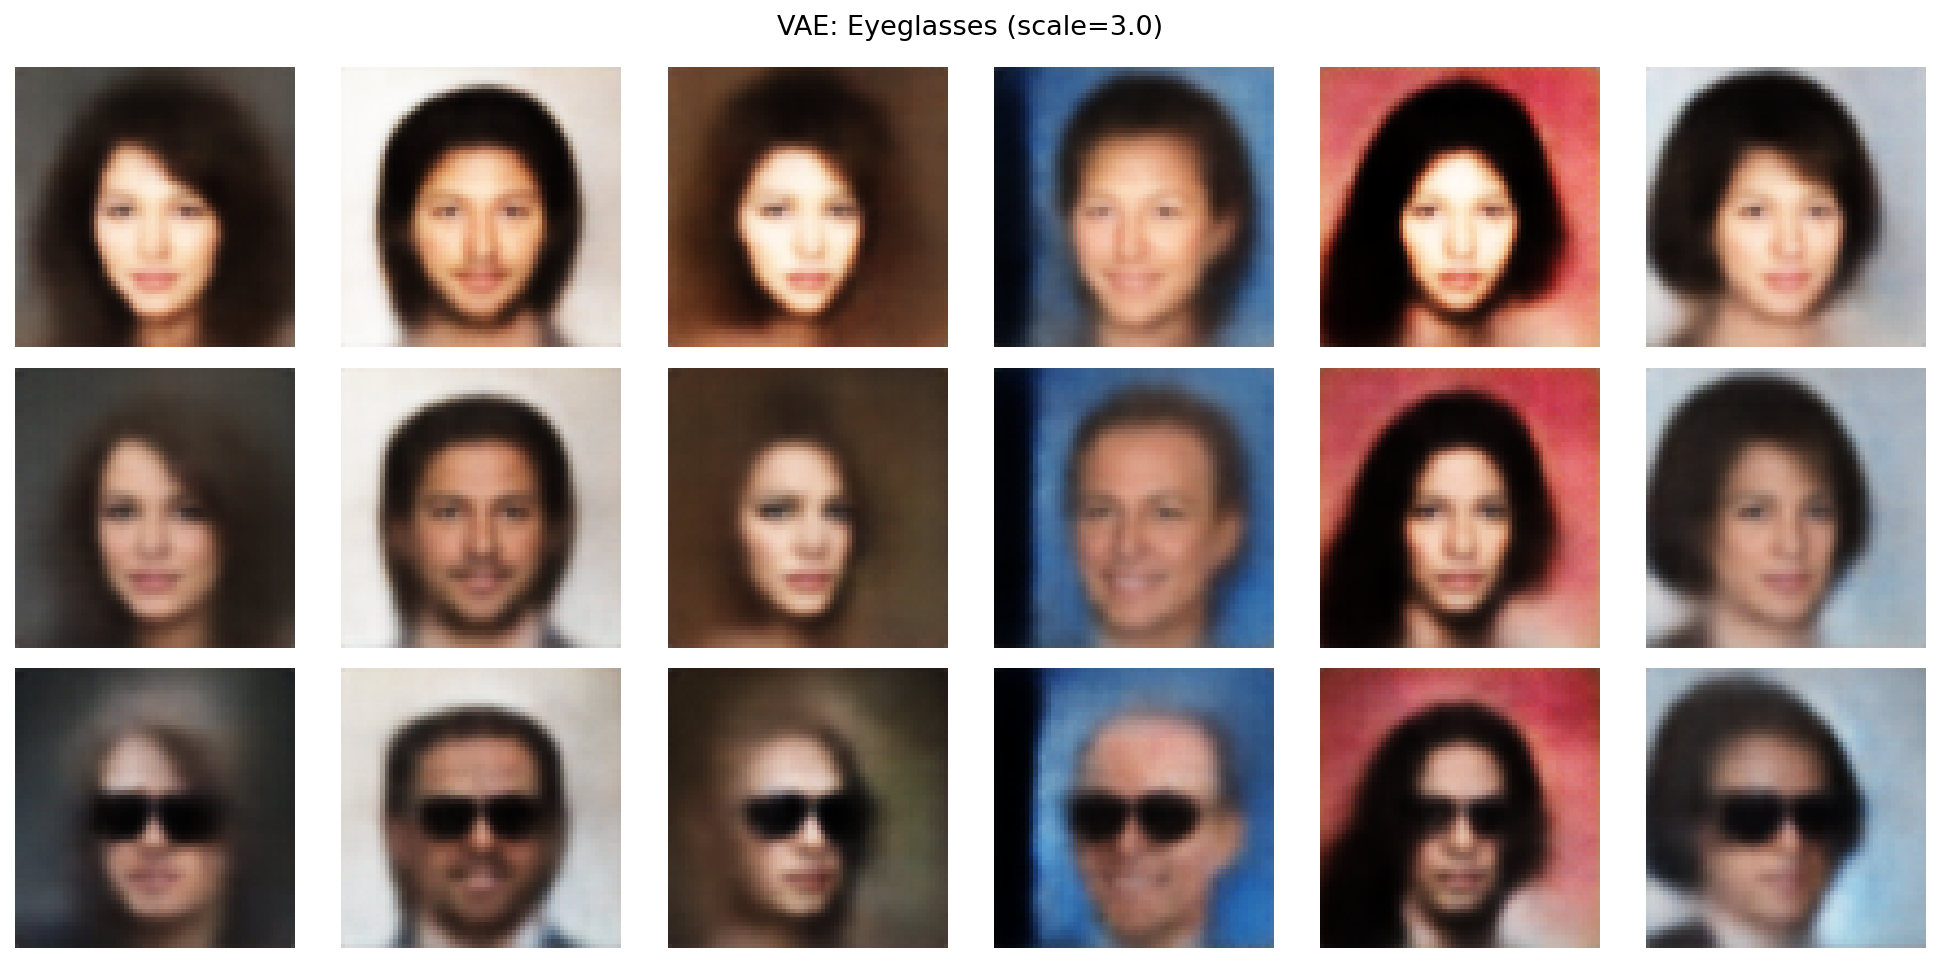
\includegraphics[width=\linewidth]{vae_attr_eyeglasses.png}
  \end{minipage}
  \caption{VAE: latent attribute shifts for \texttt{Smiling} and \texttt{Eyeglasses} (rows: $-$direction, original, $+$direction).}
\end{figure}
\begin{figure}[H]
  \centering
  \begin{minipage}{0.48\linewidth}\centering
    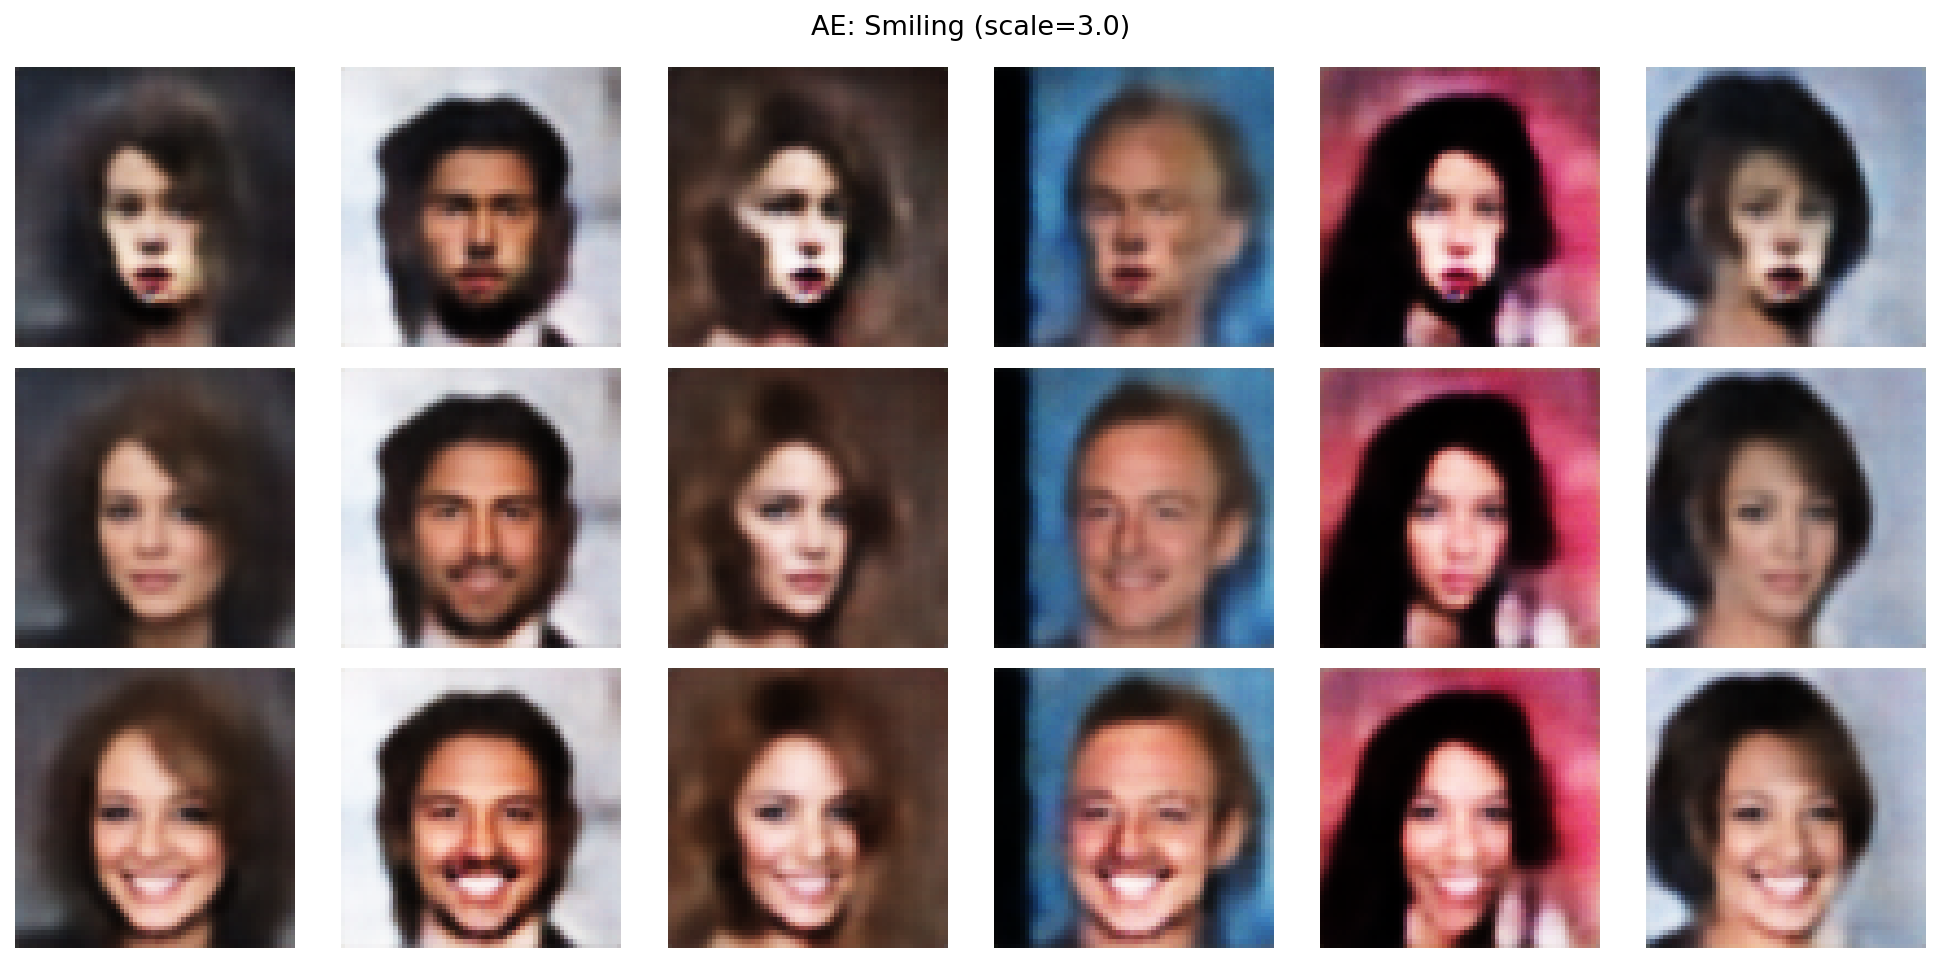
\includegraphics[width=\linewidth]{ae_attr_smiling.png}
  \end{minipage}\hfill
  \begin{minipage}{0.48\linewidth}\centering
    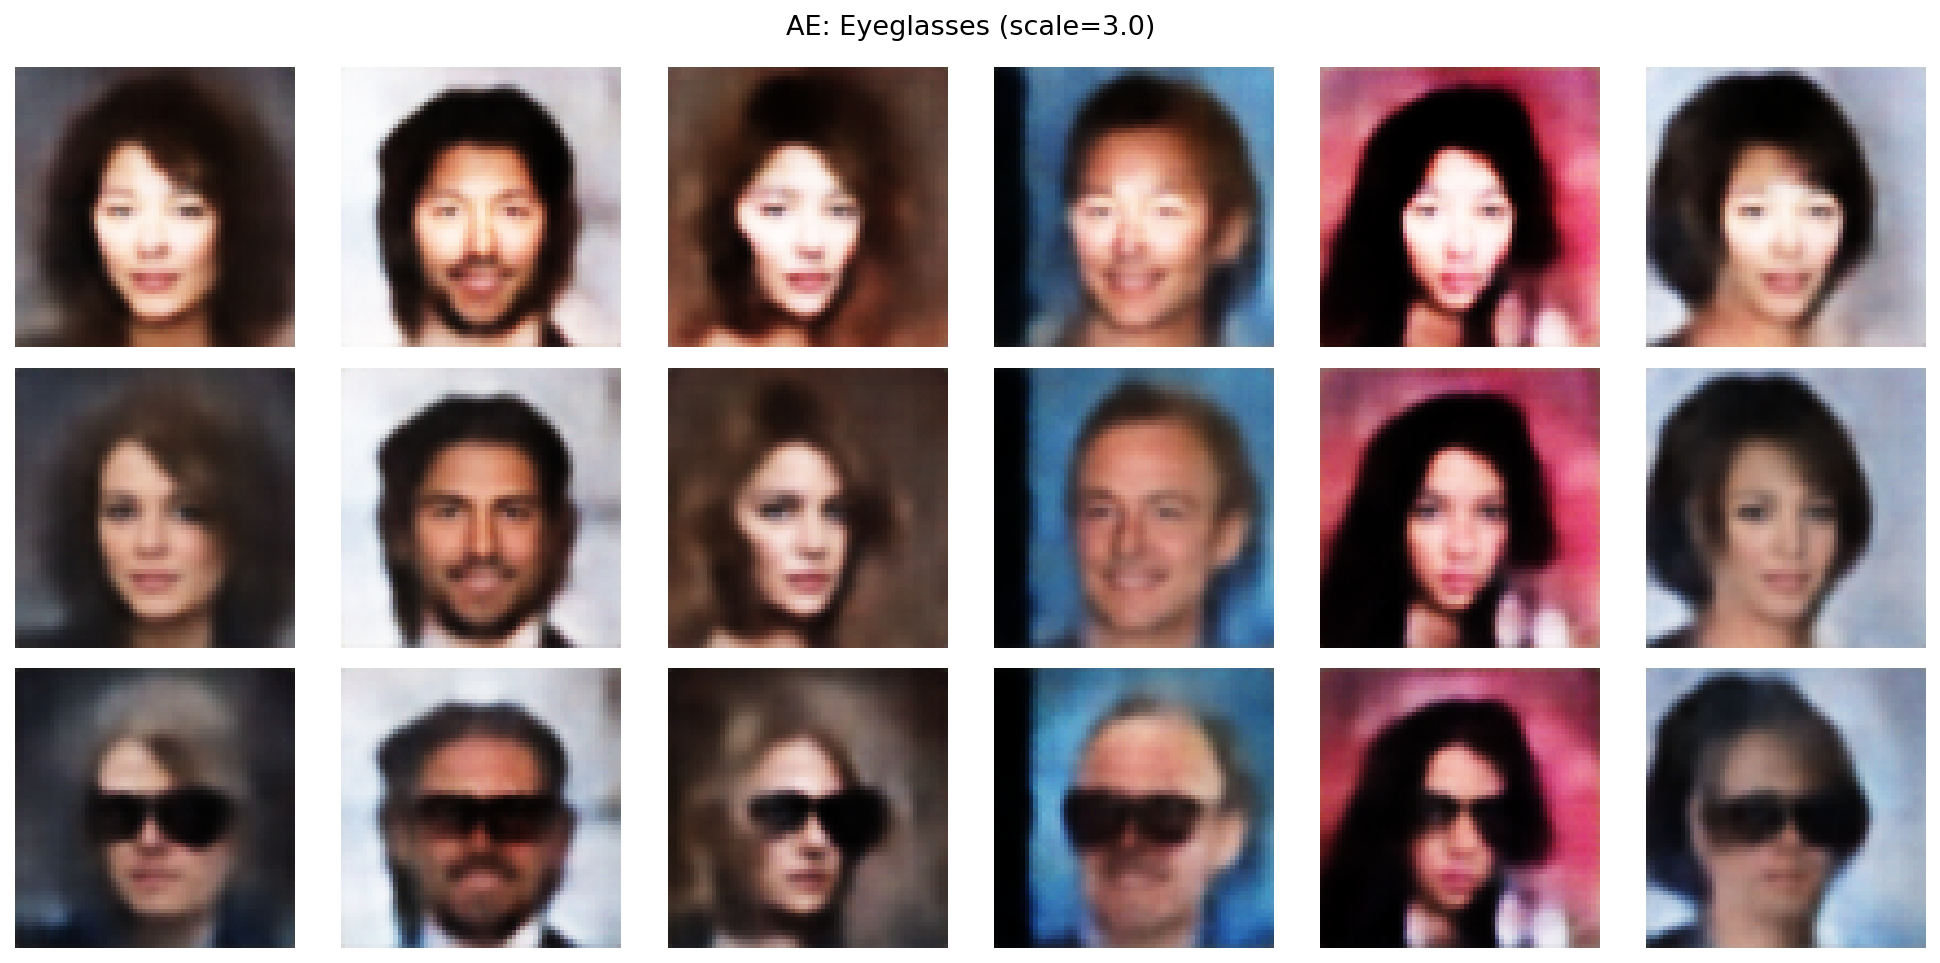
\includegraphics[width=\linewidth]{ae_attr_eyeglasses.png}
  \end{minipage}
  \caption{Standard AE: same latent attribute manipulations.}
\end{figure}
\begin{figure}[H]
  \centering
  \begin{minipage}{0.48\linewidth}\centering
    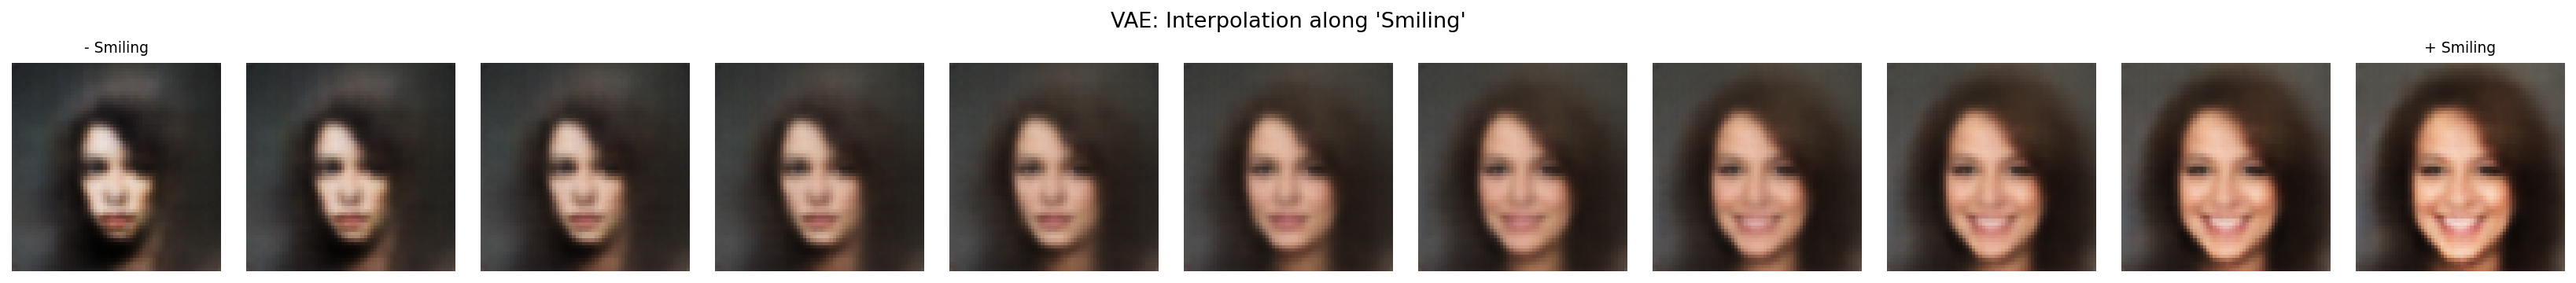
\includegraphics[width=\linewidth]{vae_interp_smiling.png}
  \end{minipage}\hfill
  \begin{minipage}{0.48\linewidth}\centering
    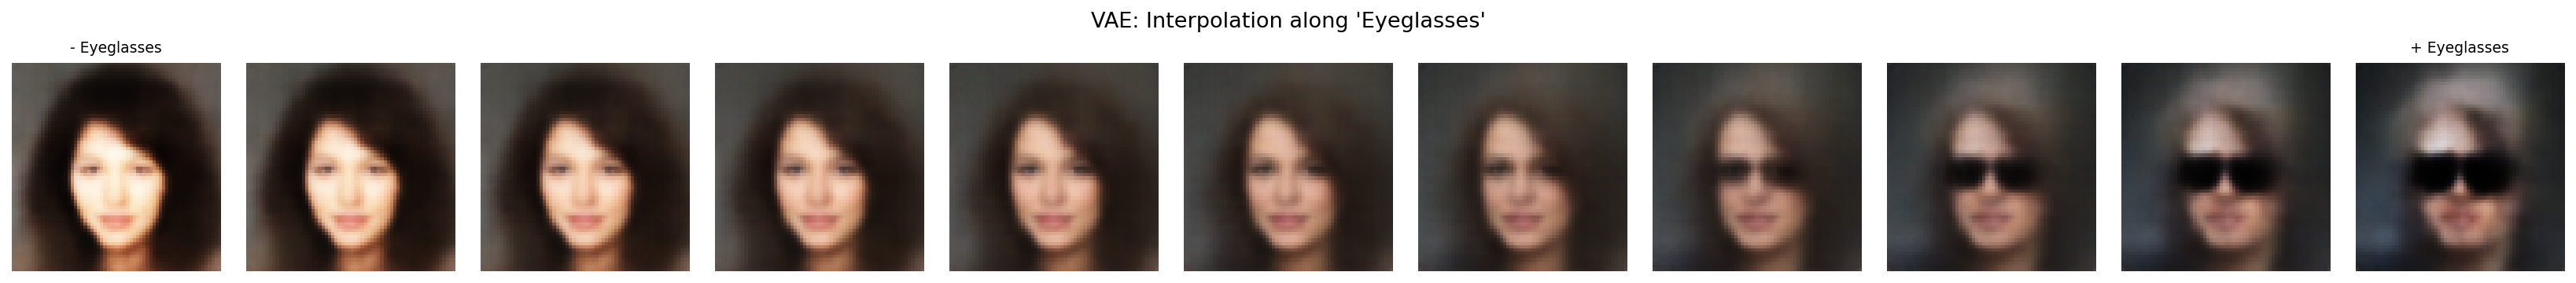
\includegraphics[width=\linewidth]{vae_interp_eyeglasses.png}
  \end{minipage}
  \caption{VAE: interpolation along the learned \texttt{Smiling} and \texttt{Eyeglasses} directions.}
\end{figure}

\end{solution}
\newpage

\begin{problem}[Decision Trees, Random Forests and Mixture of Experts]

\noindent
\begin{enumerate}
	\item Suppose we have $B$ independently trained binary classifiers (e.g., decision trees), each with the same accuracy $p > \tfrac{1}{2}$ on a given test point. The ensemble predicts by \textbf{majority vote}.

Let $X$ be the number of trees that predict correctly. Then $X \sim \text{Binomial}(B, p)$, and the ensemble is correct whenever $X > B/2$.

\medskip
\noindent
\textbf{Background: Hoeffding's Inequality.}\quad
Let $Z_1, \ldots, Z_B$ be independent random variables with $Z_i \in [a_i, b_i]$. Hoeffding's inequality states that for the sample mean $\bar{Z} = \frac{1}{B}\sum_{i=1}^{B} Z_i$:
\[
P\!\big(\bar{Z} - \mathbb{E}[\bar{Z}] \leq -t\big) \;\leq\; \exp\!\!\left(\frac{-2B^2 t^2}{\sum_{i=1}^{B}(b_i - a_i)^2}\right).
\]
Intuitively, Hoeffding's inequality is a \emph{concentration inequality}: it says that the average of many bounded independent random variables is unlikely to be far from its expectation, and this probability shrinks \emph{exponentially} in the number of samples $B$. In our setting, each $Z_i \in \{0, 1\}$ indicates whether tree $i$ is correct, so $\bar{Z} = X/B$ and $\mathbb{E}[\bar{Z}] = p$.

\begin{enumerate}
    \item \textbf{[5 points]} Apply Hoeffding's inequality to show that the ensemble error rate satisfies
    \[
    P(X \leq \tfrac{B}{2}) \leq \exp\!\Big({-2B\big(p - \tfrac{1}{2}\big)^2}\Big).
    \]
    \emph{Hint:} The ensemble errs when $\bar{Z} \leq \tfrac{1}{2}$. 

    \item \textbf{[5 points]} Compute the bound for $p = 0.6$ and $B \in \{10, 100, 1000\}$. At what $B$ does the bound first drop below $10^{-6}$? Is that good or necessary?

    \item \textbf{[5 points]} The proof above assumes the trees are \emph{independent}. In practice, bagged trees are trained on overlapping bootstrap samples and are therefore correlated.
    \begin{enumerate}
        \item Explain intuitively why correlation weakens the convergence guarantee.
        \item Random forests add \textbf{feature subsampling} (each split considers only $m$ of $d$ features at random). Explain how this reduces correlation and partially restores convergence.
    \end{enumerate}
\end{enumerate}
\item
Part 1(c) showed that correlation between trees matters. We now make this precise. Suppose we have $B$ trees $T_1, \ldots, T_B$, each with the same prediction variance $\sigma^2 = \text{Var}(T_b(\mathbf{x}))$, and each pair has the same correlation $\rho = \text{Corr}(T_i(\mathbf{x}), T_j(\mathbf{x}))$ for $i \neq j$.

\begin{enumerate}
    \item \textbf{[8 points]} Prove that the variance of the ensemble prediction is:
    \[
    \text{Var}\!\left(\frac{1}{B}\sum_{b=1}^{B} T_b(\mathbf{x})\right) = \rho\,\sigma^2 + \frac{1-\rho}{B}\,\sigma^2.
    \]
    \emph{Hint:} Expand the variance of the sum, separate the diagonal terms ($i = j$) from the off-diagonal terms ($i \neq j$), and use $\text{Cov}(T_i, T_j) = \rho\,\sigma^2$.

    \item \textbf{[4 points]} Analyze the formula:
    \begin{enumerate}
        \item What does the ensemble variance converge to as $B \to \infty$? Can we make the variance arbitrarily small by adding more trees?
        \item What happens when $\rho = 0$? When $\rho = 1$? Relate each case to a practical scenario.
    \end{enumerate}

    \item \textbf{[4 points]} Random forests use $m = \lfloor\sqrt{d}\rfloor$ features per split (for classification). Using the formula from (d), explain why $m = 1$ (one random feature per split) is generally a bad idea, even though it minimizes $\rho$. What tradeoff does $m$ control?
\end{enumerate}

%% ============================================================
\item %% ============================================================
\medskip
\noindent
\textbf{Mixture of Experts (MoE).}\quad
A random forest is a \emph{dense ensemble}: every tree processes every input. A Mixture of Experts is a \emph{sparse ensemble}: a learned gating network routes each input to only a few specialized sub-networks (``experts''), and the output is a weighted combination:
\[
y = \sum_{k=1}^{K} g_k(\mathbf{x})\, E_k(\mathbf{x}), \quad \text{with most } g_k = 0 \text{ (sparse routing)}.
\]
This is the architecture behind many modern LLMs. Sparse MoE allows models to have many more total parameters (and thus more capacity) without proportionally increasing inference cost --- for example, Mixtral 8x7B has ${\sim}47$B total parameters but activates only ${\sim}13$B per token by routing to 2 of 8 experts. Unlike random forest trees, MoE experts \emph{specialize}: the gating network learns to send different types of inputs to different experts.

A key challenge in MoE training is \textbf{expert collapse}, where the gating network funnels most inputs to one or two experts while the rest go unused, wasting capacity. This is typically addressed with an auxiliary \emph{load-balancing loss} that penalizes uneven routing.

\textbf{[4 points]} In 3--5 sentences, compare how random forests and MoE each handle the tradeoff between model capacity and computational cost. Why can a random forest not ``scale up'' in the way that MoE can?
\end{enumerate}

\end{problem}

\newpage

\begin{solution}

\paragraph{1(a).}
Let $Z_i \in \{0,1\}$ indicate whether tree $i$ is correct, so $\bar{Z} = X/B$ and $\E[\bar{Z}] = p$. The ensemble errs when at most half the trees are correct, i.e.\ $X \le B/2$, equivalently $\bar{Z} \le 1/2$. Take $t = p - \tfrac{1}{2} > 0$. Then $\bar{Z} - p \le -(p - \tfrac{1}{2})$ implies $\bar{Z} \le 1/2$. Hoeffding with $a_i = 0$, $b_i = 1$ gives $\sum_i (b_i - a_i)^2 = B$, hence
\[
  P\!\Big(\bar{Z} - p \le -\Big(p - \tfrac{1}{2}\Big)\Big)
  \le \exp\!\left(\frac{-2B^2 (p - \tfrac{1}{2})^2}{B}\right)
  = \exp\!\Big({-2B\big(p - \tfrac{1}{2}\big)^2}\Big)
\]

\paragraph{1(b).}
For $p = 0.6$, the exponent is $-2B(0.1)^2 = -0.02B$:
\[
  B = 10:\ e^{-0.2} \approx 0.82, \quad
  B = 100:\ e^{-2} \approx 0.14, \quad
  B = 1000:\ e^{-20} \approx 2.1 \times 10^{-9}
\]
We need $\exp(-0.02B) < 10^{-6}$, i.e.\ $B > \frac{\ln 10^6}{0.02} \approx 690.8$, so the first integer is $B = 691$. The bound is usually loose (conservative) because it only uses boundedness, not the binomial structure, but it still shows error probability drops exponentially in $B$ under independence.

\paragraph{1(c)(i).}
Correlated trees reuse the same mistakes: their errors cooccur, so the average does not concentrate as if we had $B$ independent bits of information.

\paragraph{1(c)(ii).}
Random subsets of features make splits in different trees depend on different dimensions, reducing pairwise correlation between trees so the ensemble mean behaves more like an average of weakly dependent (closer to independent) classifiers.

\paragraph{2(a).}
Let $S = \sum_b T_b$. Using $\mathrm{Cov}(T_i, T_j) = \rho \sigma^2$ for $i \neq j$ and $\mathrm{Var}(T_i) = \sigma^2$,
\[
  \mathrm{Var}(S) = \sum_i \mathrm{Var}(T_i) + \sum_{i \neq j} \mathrm{Cov}(T_i, T_j)
  = B\sigma^2 + B(B-1)\rho\sigma^2
\]
Thus
\[
  \mathrm{Var}\!\left(\frac{S}{B}\right)
  = \frac{\sigma^2}{B} + \frac{(B-1)\rho\sigma^2}{B}
  = \rho\sigma^2 + \frac{(1-\rho)\sigma^2}{B}
\]

\paragraph{2(b)(i).}
As $B \to \infty$, the variance tends to $\rho\sigma^2$. If $\rho > 0$, we cannot drive variance to zero with more trees alone, only reducing correlation removes the floor.

\paragraph{2(b)(ii).}
If $\rho = 0$, trees are uncorrelated and we recover the usual $O(1/B)$ averaging benefit (idealized bagging with independent bootstraps). If $\rho = 1$, all trees are identical and averaging does nothing. Variance stays $\sigma^2$, as with a single tree copied $B$ times.

\paragraph{2(c).}
$m = 1$ minimizes correlation but also starves each split of useful features, hurting bias and tree quality. The hyperparameter $m$ trades off correlation (diversity) against the chance that each split picks informative coordinates.

\paragraph{3.}
A random forest is dense, every tree evaluates every input, so doubling trees roughly doubles inference cost, capacity scales together with compute. A sparse MoE activates only a few experts per token, so total parameters (capacity) can grow large while per token FLOPs stay controlled. Random forests cannot hide most of their capacity from each prediction the way routed experts can, so they do not scale capacity and compute independently in the same sense as MoE.

\end{solution}


\newpage 




\textbf{Name}: Mert Iravul

\textbf{Collaborators and Resources}: 

\end{document}
